\documentclass{article}
\usepackage[utf8]{inputenc}
\usepackage[T1]{fontenc}
\usepackage{graphicx}
\usepackage{hyperref}
\usepackage{geometry}
\geometry{margin=1in}

\title{EXPERFILAR}
\date{Encyclopaedia Britannica (1771)}

\begin{document}
\maketitle

\section*{Historical source}
\textbf{Entry ID:} \texttt{entry-experfilar-1805} \\
\textbf{Volume ID:} 191320560 \\
\textbf{Character Count:} 560

\subsection*{Extracted Text}
EXPERFILAR, a model, or original, to be initiated, or copied. See Model.

EXEMPLAR allo denotes the idea, or image, conceived or formed in the mind of the artful, whereby he con-Kempêl did his work. Such is the idea of Center, which a painter has in his mind when he goes to make a picture of Cedar.

EXAMPILIFICATION of Letters Patents, denotes an example, or copy of letters patents, made from the embodies thereof, and falsely that the great fail of England. Such complications are as efficient to be flowered on planated, as the letters patent identifiers.



\section*{Source record}
\begin{itemize}
\item \textbf{Dataset:} \texttt{NationalLibraryOfScotland/encyclopaedia\_britannica\_illustrated}
\item \textbf{Dataset Revision:} \texttt{309f765b1ecc83e0a7f7762e44b4a927a7555443}
\item \textbf{Page ID:} \texttt{britannica:309f765b1ecc83e0a7f7762e44b4a927a7555443:train:1805} \\
  \textbf{Filename:} \texttt{page-1805-226885408318.jpg} \\
  \textbf{Row Index:} 1805 \\
  \textbf{SHA256:} \texttt{2268854083181b93...}
\end{itemize}

\begin{figure}[h]
\centering
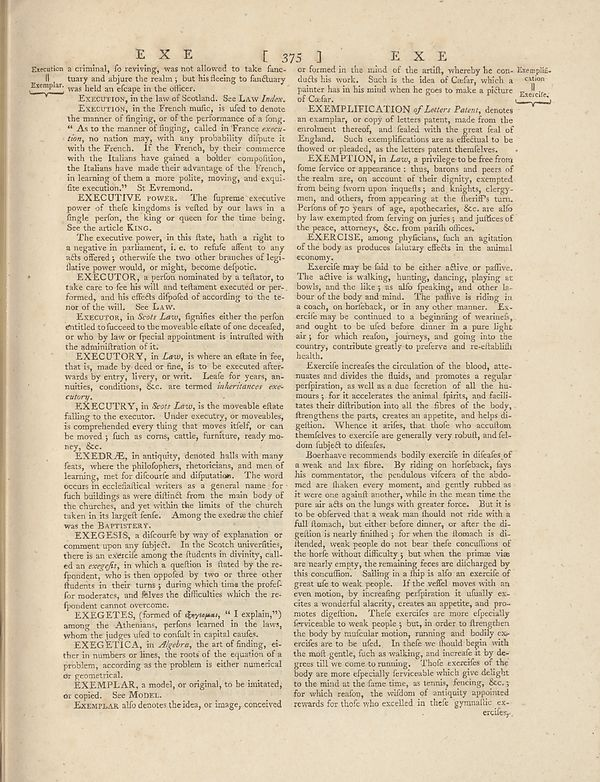
\includegraphics[width=0.85\textwidth]{../scans/page-1805-226885408318.jpg}
\caption*{Source scan: \texttt{page-1805-226885408318.jpg}}
\end{figure}

\end{document}
